\documentclass{article}
% s e l e c c i o n a e l t i p o de documento
\usepackage[spanish]{babel}
%
\usepackage[T1]{fontenc}
\usepackage[latin1]{inputenc}
\usepackage{graphicx}
\begin{document}
% i n i c i o d e l cuerpo d e l documento
\title{Laboratorio 1}
\author{Jean Carlos Chavarr\' ia Hughes B11814}
\maketitle
% t i t u l o d e l documento
\begin{abstract}
Laboratorio 4 de el curso IE 0217.
\end{abstract}
\section{Introducci\' on}
Este documento corresponde al reporte de quinto laboratorio del curso IE0217, en el cual se trabaj\' o con distintos tipos de estructuras de datos de de C++, adem\' as se practica el uso de sobrecarga de operadores, manipulaci\' on de funciones miembro, tipos de m\' etodos y funci\' on friend.

\section{Comentarios Importantes}
Para la realizaci\' on de este laboratorio se tom\' o mucho m\' as tiempo de lo esperado debido a que no se contaba con una gu\' ia para los ficheros \textit{.cpp}, de manera que se tuvo que ver los archivos \textit{.hh} para conocer que funciones debian implementarse y adem\' as ver el \textit{main} para conocer como se realizaba el llamado a las funciones.

\subsection{Clase matriz: Versi\' on 1}
La primer parte de laboratorio se realiz\' o de manera exitosa, se logr\' o dise\~ nar el m\' etodo que sumara y el que multiplicara, adem\' as de realizar la sobrecarga del constructor y los m\' etodos \textit{set()} y \textit{get()} entre otros.
Para realizar la ejecuci\' on del programa simplemente se debe proceder con la ejecuci\' on del comando \textbf{make} dentro del directorio correspondiente y luego se ejecuta el programa.
Se puede observar la ejecuci\' on del programa el la Figura \ref{fig:principal1}.
\begin{figure}[hbtp]
\caption{Principal 1}
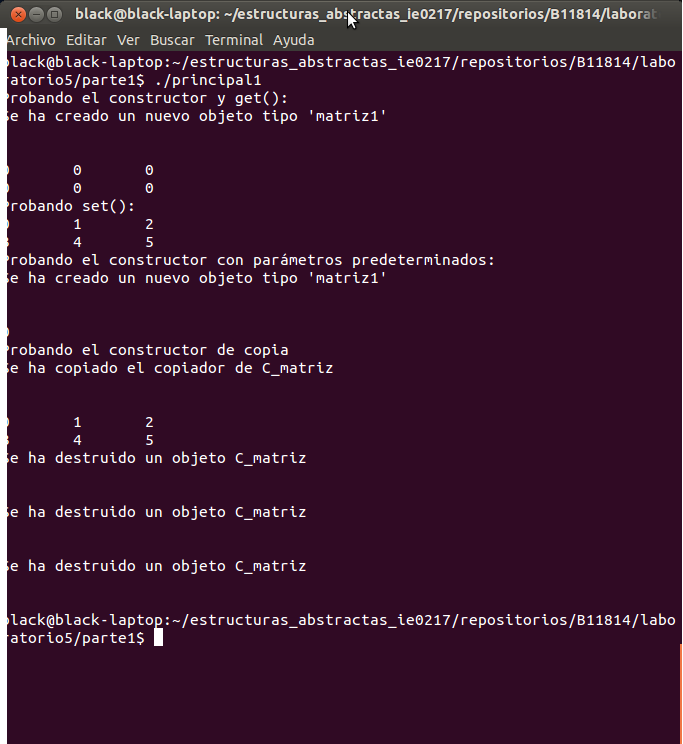
\includegraphics[scale=0.4]{./imagenes/principal1.png}
\label{fig:principal1}
\end{figure}


\subsection{Clase matriz: Versi\' on 2}
La segunda parte del laboratorio tambi\' en se ejecut\' o de manera satisfactoria, se logr\' o implementar la sobrecarga del operador (=) y otros. La ejecuci\' on es exactamente igual a la parte 1, y esta parte no demor\' o mucho tiempo debido a que era muy similar a la parte 1. 
Cabe destacar que es un error com\' un suponer que al sobrecarga un operador como el +, se sobrecargan los operadores relacionados como el +=, lo cual es incorrecto debido a que cada operador se debe sobrecarga expl\' icitamente.

La ejecuci\' on del programa se puede obsercar en la Figura \ref{fig:principal2}.

\begin{figure}[hbtp]
\caption{Principal 2}
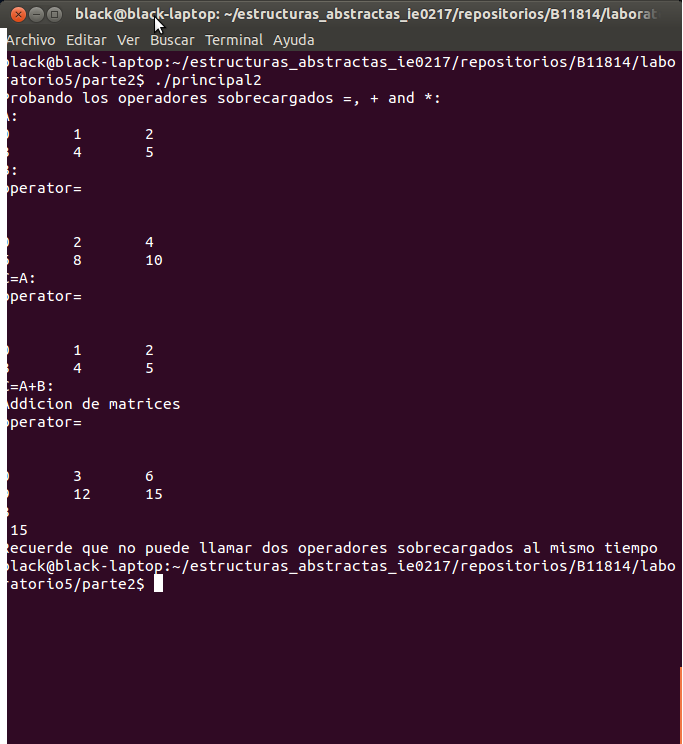
\includegraphics[scale=0.4]{./imagenes/principal2.png}
\label{fig:principal2}
\end{figure}


\subsection{Clase matriz: Versi\' on 3}
Este laboratorio tom\' o un poco m\' as de tiempo que el anterior debido a que tambi\' en se debi\' oo sobrecargar otros operadores pero con caracter\' isticas m\' as particulares y adem\' as utilizando la funci\' on amiga para algunos. Tal y como se observa en la Figura \ref{fig:principal3}.

Es posible sobrecarga un operador como una funci\' on miembro y no amiga, pero una funci\' on como esta, que necesita acceder a los datos privados o protegidos de una clase, necesitar\' ian utilizar las funciones establecer u obtener provistar en la interfaz p\' ublica de esa clase. La sobrecarga producida por llamar a estas funciones podr\' ia ocasionar un rendimiento deficiente, por lo que se puede hacer que estas funciones sean \textbf{inline}  para mejorar el rendimiento.

\begin{figure}[hbtp]
\caption{Principal 3}
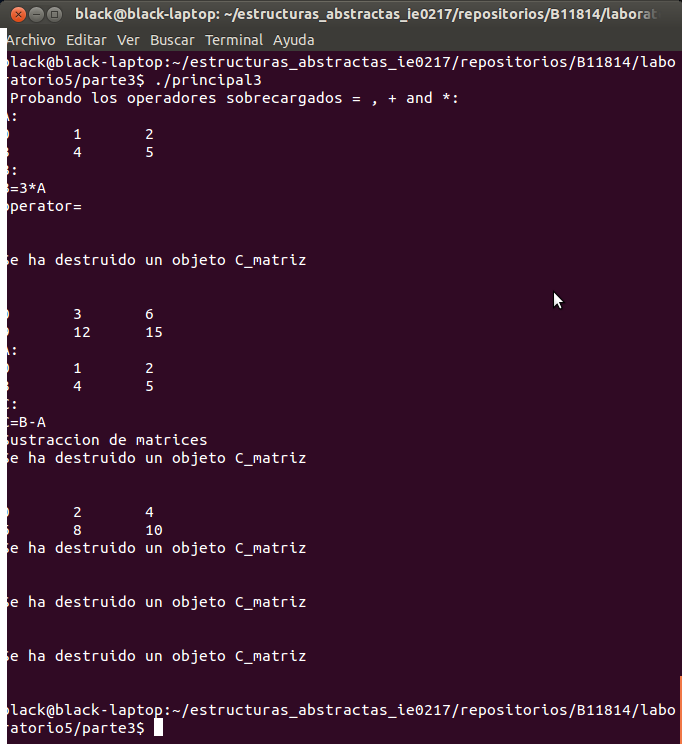
\includegraphics[scale=0.4]{./imagenes/principal3.png}
\label{fig:principal3}
\end{figure}




\end{document}
